\section{Difa Al Fansha (1174076)}
\subsection{Menulis dan membaca shapefile}
\begin{enumerate}
\item Nomor 1
	\lstinputlisting{src/tugas2/1174076/soal1.py}
	\begin{figure}[H]
	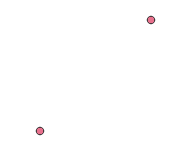
\includegraphics[width=6cm]{figures/Tugas2/1174076/soal1.png}
		\centering
		\caption{Nomor 1 Point (Titik)}
	\end{figure}
	
	\item Nomor 2
	\lstinputlisting{src/tugas2/1174076/soal2.py}
	\begin{figure}[H]
		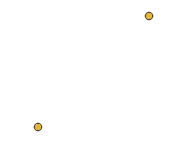
\includegraphics[width=6cm]{figures/Tugas2/1174076/soal2.png}
		\centering
		\caption{Nomor 2 Point (Titik)}
	\end{figure}
	
	\item Nomor 3
	\lstinputlisting{src/tugas2/1174076/soal3.py}
	\begin{figure}[H]
		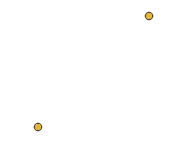
\includegraphics[width=6cm]{figures/Tugas2/1174076/soal3.png}
		\centering
		\caption{Nomor 3 Point (Titik)}
	\end{figure}
	
	\item Nomor 4
	\lstinputlisting{src/tugas2/1174076/soal4.py}
	\begin{figure}[H]
		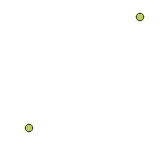
\includegraphics[width=6cm]{figures/Tugas2/1174076/soal4.png}
		\centering
		\caption{Nomor 4 Point (Titik)}
	\end{figure}

	\item Nomor 5
	\lstinputlisting{src/tugas2/1174076/soal5.py}
	\begin{figure}[H]
		
\includegraphics[width=6cm]{figures/Tugas2/1174076/soal5.png}
		\centering
		\caption{Nomor 5 Garis}
	\end{figure}

	\item Nomor 6
	\lstinputlisting{src/tugas2/1174076/soal6.py}
	\begin{figure}[H]
		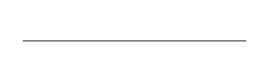
\includegraphics[width=6cm]{figures/Tugas2/1174076/soal6.png}
		\centering
		\caption{Nomor 6 Garis lurus}
	\end{figure}

	\item Nomor 7
	\lstinputlisting{src/tugas2/1174076/soal7.py}
	\begin{figure}[H]
		
\includegraphics[width=6cm]{figures/Tugas2/1174076/soal7.png}
		\centering
		\caption{Nomor 7 Jam Pasir}
	\end{figure}

	\item Nomor 8
	\lstinputlisting{src/tugas2/1174076/soal8.py}
	\begin{figure}[H]
		
\includegraphics[width=6cm]{figures/Tugas2/1174076/soal8.png}
		\centering
		\caption{Nomor 8 Jam Pasir}
	\end{figure}

	\item Nomor 9
	\lstinputlisting{src/tugas2/1174076/soal9.py}
	\begin{figure}[H]
		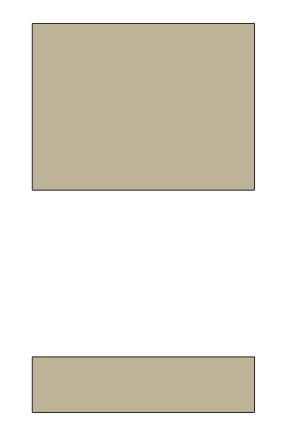
\includegraphics[width=6cm]{figures/Tugas2/1174076/soal9.png}
		\centering
		\caption{Nomor 9 Kotak dan Persegi Panjang}
	\end{figure}

	\item Nomor 10
	\lstinputlisting{src/tugas2/1174076/soal10.py}
	\begin{figure}[H]
		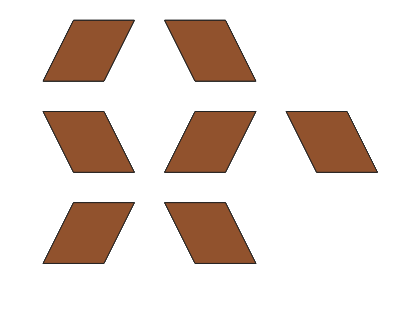
\includegraphics[width=6cm]{figures/Tugas2/1174076/soal10.png}
		\centering
		\caption{Nomor 10 Jajar Genjang}
	\end{figure}
Rumus mencari soal: 117076 MOD 8 = 4\\ 
Disini saya mengerjakan soal nomor 4, yaitu membuat jajar genjang \\
Karna dua digit 7 saya membuat jajar genjang sebanyak 7 buah
\end{enumerate}

\subsection{Link}
https://youtu.be/2SusnHVlTYA